\documentclass{ximera}

\input{../preamble.tex}

\outcome{Use reduction formulas and the Pythagorean identity to compute
  integrals involving trigonometric functions.}
\outcome{Recognize the patterns that appear in trigonometric integrals,
  and use appropriate substitutions to compute them.}
\outcome{Compute integrals involving powers of sine and cosine.}

\title[Dig-In:]{Trigonometric integrals}

\begin{document}
\begin{abstract}
  We can substitution and trigonometric identities to antidifferentiate
  trigonometric functions.
\end{abstract}
\maketitle

Here are some strategies for dealing with expressions of the following
form:
\[
\int \sin^n(x)\cos^m(x) \d x
\]
Functions like these, consisting of products of sine and cosine, can
be antidifferentiated by using substitution and trigonometric
identities. This process can be tedious, but the idea is
straightforward. The basic idea in each case is to somehow take
advantage of a trigonometric identity, usually the \dfn{Pythagorean
  identity}:
\[
\cos^2(x) + \sin^2(x) = 1
\]

\section{If either power is odd}

\begin{example}
  Compute:
  \[
  \int \sin^5(x) \cos^2(x) \d x
  \]
  \begin{explanation}
    Since the power of sine is odd, we can rewrite this suggestively as
    \begin{align*}
    \int &\sin^4(x) \cos^2(x) \sin(x) \d x \\
    &= \int (\sin^2x)^2 \cos^2(x) \sin(x) \d x
    \end{align*}
    Now using the Pythagorean identity we can rewrite everything in
    terms of $\cos(x)$, but reserve the one power of $\sin(x)$ to help
    with the differential in an eventual variable substitution:
    \begin{center}%% used center instead of image since there is no reason for a LARGE integral in the text
      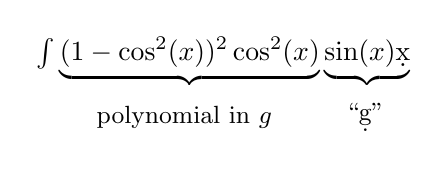
\begin{tikzpicture}
        \node at (0,0) {
          $\int \underbrace{(1-\cos^2(x))^2 \cos^2(x)} \underbrace{\sin(x) \d x}$
        };
        \node at (-.5,-.7) {\small{polynomial in $g$}};
        \node at (1.8,-.7) {\small{``$\d g$''}};
      \end{tikzpicture}
    \end{center}
    Making the substitution
    \begin{align*}
      g &= \cos(x)\\
      \d g &=\answer[given]{-\sin(x)} \d x
    \end{align*}
    yields
    \[
    \int \answer[given]{-(1-g^2)^2 g^2} \d g
    \]
    This is a polynomial in $g$, and so we can easily finish the
    integration by just expanding the polynomial out and integrating
    term-by-term. Write with me
    \begin{align*}
      \int {-(1-g^2)^2 g^2} \d g &= \int -(1-2g^2+g^4)g^2\d g\\
      &= \int-g^6 + 2g^4-g^2 \d g\\
      &=\answer[given]{-g^7/7 + 2g^5/5 - g^3/3}+C
    \end{align*}
    Substituting $g = \cos(x)$ we find our final answer:
    \[
    -\cos^7(x)/7 + 2\cos^5(x)/5 - \cos^3(x)/3+C
    \]
  \end{explanation}
\end{example}

We can generalize this thinking whenever we have an odd-power:

\subsection{Odd powers of sine}

If we are integrating a product of powers of sine and cosine
functions, and the power of sine is odd, then the integral looks like
\[
\int \sin^{2k+1}(x) \cos^m(x) \d x
\]
where $k$ is some integer.  Then
\begin{align*}
  \int \sin^{2k+1}(x) \cos^m(x) \d x &=\int(\sin^{2}(x))^k \cos^m(x) \sin(x) \d x\\
  &= \int (1-\cos^2(x))^k \cos^m(x) \sin(x)\d x.
\end{align*}
We have now set ourselves up for an eventual substitution:
\begin{center}%% used center instead of image since there is no reason for a LARGE integral in the text
  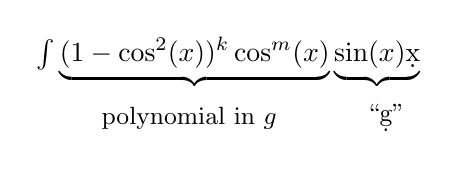
\begin{tikzpicture}
    \node at (0,0) {
      $\int \underbrace{(1-\cos^2(x))^k \cos^m(x)} \underbrace{\sin(x) \d x}$
        };
    \node at (-.5,-.7) {\small{polynomial in $g$}};
    \node at (2,-.7) {\small{``$\d g$''}};
  \end{tikzpicture}
\end{center}
so letting $g = \cos(x)$ so $\d g =-\sin(x) \d x$, we have
\[
\int -(1-g^2)^k g^m \d g
\]
which is a polynomial, and can be integrated term-by-term after
expansion.


\begin{question}
  Consider the following integral:
  \[
  \int \sec^{27}(x)\csc^{83}(x) \d x
  \]
  After making the substitution, $g = \cos(x)$ we find
  \begin{hint}
    First express secant and cosecant in terms of cosine and sine.
  \end{hint}\begin{multipleChoice}
    \choice{$\int -(1-g^2)^{13} g^{83} \d g$}
    \choice{$\int -(1-g^2)^{27} g^{83} \d g$}
    \choice[correct]{$\int -(1-g^2)^{-42} g^{-27} \d g$}
    \choice{$\int -(1-g^2)^{-27} g^{-42} \d g$}
  \end{multipleChoice}
\end{question}



\subsection{Odd powers of cosine}

We can follow exactly the same line of thinking in this case. If we
are integrating a product of powers of sine and cosine, and the power
of cosine is odd, then the integral looks like
\[
\int \sin^n(x) \cos^{2k+1}(x) \d x
\]
where $k$ is some integer. Then
\begin{align*}
\int \sin^n(x) \cos^{2k+1}(x) \d x &=\int \sin^n(x) (\cos^{2}(x))^k \cos(x)\d x\\
&= \int \sin^n(x) (1-\sin^{2}(x))^k \cos(x) \d x.
\end{align*}
We have now set ourselves up for an eventual substitution:
\begin{center}%% used center instead of image since there is no reason for a LARGE integral in the text
  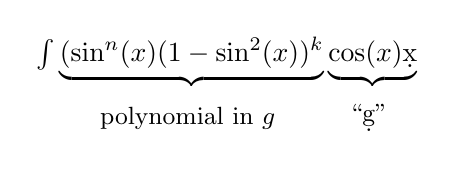
\begin{tikzpicture}
    \node at (0,0) {
      $\int \underbrace{( \sin^n(x) (1-\sin^{2}(x))^k} \underbrace{\cos(x) \d x}$
        };
    \node at (-.5,-.7) {\small{polynomial in $g$}};
    \node at (1.8,-.7) {\small{``$\d g$''}};
  \end{tikzpicture}
\end{center}
so letting $g = \sin(x)$ so $\d g =\cos(x) \d x$, we have 
\[
\int g^n(1-g^2)^k \d g
\]
which is a polynomial, and can be integrated term-by-term after
expansion.

\begin{question}
  Consider the following integral:
  \[
  \int \sec^{90}(x) \cot^{59}(x)  \d x
  \]
  After making the substitution, $g = \sin(x)$ we find
  \begin{hint}
    First express secant and cosecant in terms of cosine and sine.
  \end{hint}
  \begin{multipleChoice}
    \choice[correct]{$\int g^{-59}(1-g^2)^{-16} \d g$}
    \choice{$\int g^{90}(1-g^2)^{29} \d g$}
    \choice{$\int g^{29}(1-g^2)^{90} \d g$}
    \choice{$\int g^{-18}(1-g^2)^{-59} \d g$}
  \end{multipleChoice}
\end{question}


\begin{warning}
Instead of memorizing this general result, you should focus on
internalizing the \textbf{process} by which the result was obtained.
In each case,
\begin{itemize}
\item you take off one power of a trigonometric function, and
\item you are left with an even power of that trigonometric
  function.
\end{itemize}
You can then use a Pythagorean identity to rewrite that even power in
terms of the other trigonometric functions.  Making a variable
substitution finishes the conversion to a polynomial function (or as
we will see, a rational function) in $g$.
\end{warning}



Sometimes we need to massage our function into the correct form:

\begin{example}
  Compute:
  \[
  \int \sin^5(x) \d x
  \]
  \begin{explanation}
    Write with me, we start by separating a power of sine for an eventual substitution
    \begin{align*}
      \int \sin^5 x\d x &=\int \sin^4(x) \sin(x) \d x\\
      &=\int (\sin^2(x))^2 \sin(x) \d x
    \end{align*}
    Here is what we're thinking:
    \begin{center}%% used center instead of image since there is no reason for a LARGE integral in the text
      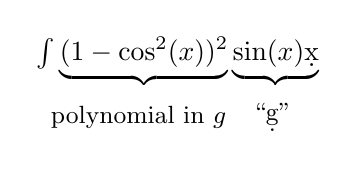
\begin{tikzpicture}
        \node at (0,0) {
          $\int \underbrace{(1-\cos^2(x))^2} \underbrace{\sin(x) \d x}$
        };
        \node at (-.5,-.7) {\small{polynomial in $g$}};
        \node at (1.2,-.7) {\small{``$\d g$''}};
      \end{tikzpicture}
    \end{center}
    Now set $g=\cos x$, $\d g=-\sin x\d x$:
    \begin{align*}
      \int \sin x (1-\cos^2 x)^2\d x&=\int \answer[given]{-(1-g^2)^2} \d g \\
      &=\int -(1-2g^2+g^4)\d g \\
      &=\answer[given]{-g+\frac{2}{3}g^3-\frac{1}{5}g^5}+C
    \end{align*}
    Hence our final answer is:
    \[
    \answer[given]{-\cos x+\frac{2}{3}\cos^3 x-\frac{1}{5}\cos^5x}+C
    \]
  \end{explanation}
\end{example}


\subsection{Working with other trigonometric functions}

A general strategy for dealing with trigonometric integrals is to
express every trigonometric function in terms of cosine and sine, and
then proceed as we have above. However, this is not the only trick up
our sleeve.  Remember, the Pythagorean identity has two other forms:
\[
1 + \tan^2(x) = \sec^2(x) \qquad\text{and}\qquad \cot^2(x) + 1 = \csc^2(x)
\]
the first identity we find by dividing the Pythagorean identity by
$\cos^2(x)$ and the second we find by dividing by $\sin^2(x)$. It is
worth seeing several examples where we use these identities.



\begin{example}
  Compute
  \[
  \int \tan^3(x) \sec^4(x) \d x
  \]
  \begin{explanation}
    Since the power of secant is even, we can rewrite this suggestively as
    \begin{align*}
    \int &\tan^3(x) \sec^4(x) \d x \\
    &= \int\tan^3(x) \sec^2(x) \sec^2(x) \d x
    \end{align*}
    Now using the Pythagorean identity we can rewrite everything in
    terms of $\tan(x)$, but reserve the one power of $\sec^2(x)$ to help
    with the differential in an eventual variable substitution:
    \begin{center}%% used center instead of image since there is no reason for a LARGE integral in the text
      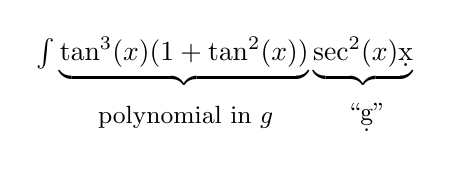
\begin{tikzpicture}
        \node at (0,0) {
          $\int \underbrace{\tan^3(x)(1+\tan^2(x))} \underbrace{\sec^2(x) \d x}$
        };
        \node at (-.5,-.7) {\small{polynomial in $g$}};
        \node at (1.8,-.7) {\small{``$\d g$''}};
      \end{tikzpicture}
    \end{center}
    Making the substitution
    \begin{align*}
      g &= \tan(x)\\
      \d g &=\answer[given]{\sec^2(x)} \d x
    \end{align*}
    yields
    \[
    \int \answer[given]{g^3(1+g^2)} \d g
    \]
    This is a polynomial in $g$, and so we can easily finish the
    integration by just expanding the polynomial out and integrating
    term-by-term. We leave it to the intrepid young mathematician to
    finish this problem.
  \end{explanation}
\end{example}


\begin{example}
  Compute
  \[
  \int \tan^3(x) \sec^5(x) \d x
  \]
  \begin{explanation}
    Since the power of tangent is odd and the power of secant is odd,
    we can rewrite this suggestively as
    \begin{align*}
    \int &\tan^3(x) \sec^5(x) \d x \\
    &= \int\tan^2(x) \sec^4(x) \sec(x)\tan(x) \d x
    \end{align*}
    Now using the Pythagorean identity we can rewrite everything in
    terms of $\sec(x)$, but reserve the one power of $\sec(x)\tan(x)$ to help
    with the differential in an eventual variable substitution:
    \begin{center}%% used center instead of image since there is no reason for a LARGE integral in the text
      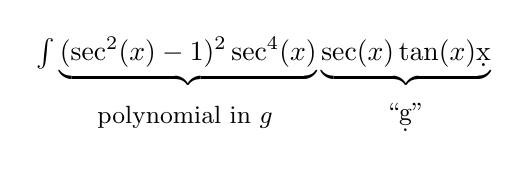
\begin{tikzpicture}
        \node at (0,0) {
          $\int \underbrace{(\sec^2(x)-1)^2\sec^4(x)} \underbrace{\sec(x)\tan(x) \d x}$
        };
        \node at (-1,-.7) {\small{polynomial in $g$}};
        \node at (1.8,-.7) {\small{``$\d g$''}};
      \end{tikzpicture}
    \end{center}
    Making the substitution
    \begin{align*}
      g &= \sec(x)\\
      \d g &=\answer[given]{\sec(x)\tan(x)} \d x
    \end{align*}
    yields
    \[
    \int \answer[given]{(g^2-1)^2g^4} \d g
    \]
    This is a polynomial in $g$, and so we can easily finish the
    integration by just expanding the polynomial out and integrating
    term-by-term. We leave it to the interested young mathematician to
    finish this problem.
  \end{explanation}
\end{example}


Let's do some problems involving cotangent and cosecant for
completeness sake.

\begin{example}
  Compute
  \[
  \int \cot^3(x) \csc^4(x) \d x
  \]
  \begin{explanation}
    Since the power of cotangent is odd and the power of cosecant is even,
    we can rewrite this suggestively as
    \begin{align*}
      \int &\cot^3(x) \csc^4(x) \d x \\
    &= \int\cot^3(x) \csc^2(x) \csc^2(x) \d x
    \end{align*}
    Now using the Pythagorean identity we can rewrite everything in
    terms of $\cot(x)$, but reserve the one power of $\csc^2(x)$ to help
    with the differential in an eventual variable substitution:
    \begin{center}%% used center instead of image since there is no reason for a LARGE integral in the text
      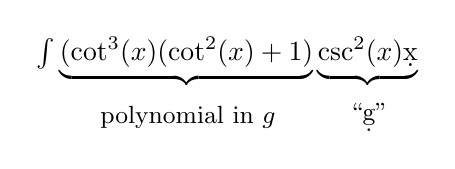
\begin{tikzpicture}
        \node at (0,0) {
          $\int \underbrace{(\cot^3(x)(\cot^2(x)+1)} \underbrace{\csc^2(x) \d x}$
        };
        \node at (-.5,-.7) {\small{polynomial in $g$}};
        \node at (1.8,-.7) {\small{``$\d g$''}};
      \end{tikzpicture}
    \end{center}
    Making the substitution
    \begin{align*}
      g &= \cot(x)\\
      \d g &=\answer[given]{-\csc^2(x)} \d x
    \end{align*}
    yields
    \[
    \int \answer[given]{-g^3(g^2+1)} \d g
    \]
    This is a polynomial in $g$, and so we can easily finish the
    integration by just expanding the polynomial out and integrating
    term-by-term. We leave it to the fearless young mathematician to
    finish this problem.
  \end{explanation}
\end{example}



\begin{example}
  Compute
  \[
  \int \cot^3(x) \csc^5(x) \d x
  \]
  \begin{explanation}
    Since the power of cotangent is odd and the power of cosecant is
    odd, we can rewrite this suggestively as
    \begin{align*}
      \int &\cot^3(x) \csc^5(x) \d x \\
    &= \int\cot^2(x) \csc^4(x) \csc(x)\cot(x) \d x
    \end{align*}
    Now using the Pythagorean identity we can rewrite everything in
    terms of $\csc(x)$, but reserve the one power of $\csc(x)\cot(x)$ to help
    with the differential in an eventual variable substitution:
    \begin{center}%% used center instead of image since there is no reason for a LARGE integral in the text
      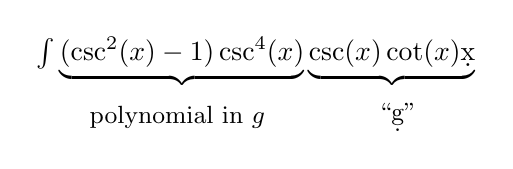
\begin{tikzpicture}
        \node at (0,0) {
          $\int \underbrace{(\csc^2(x)-1)\csc^4(x)} \underbrace{\csc(x)\cot(x) \d x}$
        };
        \node at (-1,-.7) {\small{polynomial in $g$}};
        \node at (1.8,-.7) {\small{``$\d g$''}};
      \end{tikzpicture}
    \end{center}
    Making the substitution
    \begin{align*}
      g &= \csc(x)\\
      \d g &=\answer[given]{-\csc(x)\cot(x)} \d x
    \end{align*}
    yields
    \[
    \int \answer[given]{-(g^2-1)g^4} \d g
    \]
    This is a polynomial in $g$, and so we can easily finish the
    integration by just expanding the polynomial out and integrating
    term-by-term. We leave it to the patient young mathematician to
    finish this problem.
  \end{explanation}
\end{example}




\section{When both powers are even}

Thinking again about powers of cosine and sine, what do we do when
both powers are even?  Our strategy above is sunk, since peeling-off
one power leaves an odd power, and we cannot use the Pythagorean
identity to rewrite this in a nice way.  Instead, we will use the
power-reduction formulas:

\begin{description}\index{power-reduction}
\item[Cosine Power-Reduction] $\cos^2(x)= \frac{1+\cos(2x)}{2}$\index{cosine power-reduction}
\item[Sine Power-Reduction] $\sin^2(x) = \frac{1-\cos(2x)}{2}$\index{sine power-reduction}
\end{description}

In this case, it is (usually) critical to apply the power-reduction
formulas to \textit{every} instance of cosine and sine appearing in
the integrand.

\begin{example}
  Compute:
  \[
  \int \sin^2x\cos^2x\d x
  \]
  \begin{explanation} 
    Use both power-reduction formulas to find:
    \[
    \int \sin^2x\cos^2x\d x=\int \frac{1-\cos(2x)}{2}\cdot
    \frac{1+\cos(2x)}{2}\d x
    \]
    From here, we can try to simplify further.  We may end up having
    to use either of these strategies multiple times.  In this case
    \begin{align*}
      \int \frac{1-\cos(2x)}{2} \cdot \frac{1+\cos(2x)}{2}\d x &= \frac{1}{4} \int 1-\cos^2(2x) \d x\\
      &= \frac{1}{4} \int \sin^2(2x) \d x
    \end{align*}
    
    Since this expression has only even powers of sine, we must use
    the same strategy again, and employ a power-reduction formula:
    \[
    \sin^2(2x) = \frac{1-\cos(\answer[given]{4x})}{2}
    \]
    so we find
    \[
    \frac{1}{8}\int 1-\cos(4x) \d x = \answer[given]{\frac{1}{8}(x - \frac{1}{4}\sin(4x))} + C
    \]
  \end{explanation}
\end{example}


\section{Antiderivatives of other trigonometric functions}

Finally we will reveal the antiderivatives of functions like secant,
cosecant, tangent, and cotangent.

\begin{example}
  Compute:
  \[
  \int \sec (x) \d x
  \]
  \begin{explanation}
    Write with me
    \begin{align*}
      \int \sec(x) \d x &= \int \cos(x)^{-1} \d x\\
      &= \int \cos^{-2}(x)\cos(x) \d x\\
      &=\int(1-\sin^2(x))^{-1} \cos(x) \d x
    \end{align*}
    We have now set ourselves up for an eventual substitution:
    \begin{center}%% used center instead of image since there is no reason for a LARGE integral in the text
      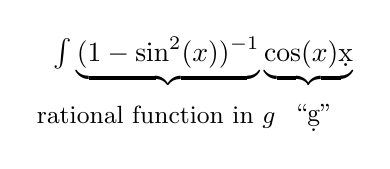
\begin{tikzpicture}
        \node at (0,0) {
          $\int \underbrace{(1-\sin^2(x))^{-1}} \underbrace{\cos(x) \d x}$
        };
        \node at (-.6,-.7) {\small{rational function in $g$}};
        \node at (1.4,-.7) {\small{``$\d g$''}};
      \end{tikzpicture}
    \end{center}
    Set $g =\sin(x)$ so $\d g = \cos(x) \d x$, and write with me
    \begin{align*}
      \int(1-\sin^2(x))^{-1} \cos(x) \d x &= \int \frac{1}{1-g^2}\d g\\
      &= \frac{1}{2}\int \frac{1}{1-g} + \frac{1}{1+g} \d g\
    \end{align*}
    Antidifferentiating we find
    \begin{align*}
      &=\frac{1}{2}\left(\ln(1-g) - \ln(1-g)\right)+C\\
      &= \frac{1}{2}\ln\left(\frac{1+\sin(x)}{1-\sin(x)}\right)+C
    \end{align*}
    Note, we could stop here, but we won't because this is not the
    typical antiderivative of $\sec(x)$. Please keep writing with me
    \begin{align*}
      \frac{1}{2}\ln\left(\frac{1+\sin(x)}{1-\sin(x)}\right)+C &= \frac{1}{2}\ln\left(\frac{(1+\sin(x))^2}{1-\sin^2(x)}\right)+C \\
      &= \frac{1}{2}\ln\left(\frac{(1+\sin(x))^2}{\cos^2(x)}\right)+C \\
      &= \ln\left(\frac{1+\sin(x)}{\cos(x)}\right)+C \\
      &= \ln\left|\sec(x) + \tan(x)\right|+C \\
    \end{align*}
  \end{explanation}
\end{example}

Using a similar technique, we can find the antiderivatives of other trigonometric functions:


\begin{theorem}[Antiderivatives of trigonometric functions]\hfil
  \begin{itemize}
  \item $\int \tan(x) \d x = -\ln|\cos(x)| + C$
  \item $\int \cot(x) \d x = \ln|\sin(x)| + C$
  \item $\int \sec(x) \d x = \ln|\sec(x) + \tan(x)| + C$
  \item $\int \csc(x) \d x = -\ln|\csc(x) + \cot(x)| + C$
  \end{itemize}
\end{theorem}



\subsection{Summary}

So when confronted with even powers of both sine and cosine, we employ
the power-reduction formulas, simplify, and see what we end up with.
If we get some odd powered terms, we can use that strategy for those
parts.  If we end up with both even powers again, we might have to use
this strategy multiple times.  This can get tricky algebraically, but
if you are careful, you will eventually emerge victorious.


\end{document}

